
\documentclass{article}[11pt]

\usepackage[utf8]{inputenc}
\usepackage[margin=1in]{geometry}
 \usepackage{setspace} \onehalfspacing
\setlength\parindent{0pt}
\setlength{\parskip}{1em}
\setcounter{secnumdepth}{0}
\usepackage{outlines}
\usepackage{graphicx}
\usepackage{caption}
\captionsetup{justification=centering, width=5in}
\graphicspath{ {imgs} }
\usepackage[normalem]{ulem}
\usepackage{hyperref}
\usepackage{color,soul}

\usepackage{comment}
\pagenumbering{gobble}

\usepackage[
backend=biber,
style=apa,
citestyle=authoryear,
sorting=nyt,
]{biblatex}
\addbibresource{photo_essay.bib}

\title{Ninoofsepoort, an opportunity lost to capital?}
\author{Carla Hyenne}
\date{}

\begin{document}

\newgeometry{margin=0.5in, top=1in}

\maketitle

\begin{figure}[h!]
	\centering
	\captionsetup{labelformat=empty}
	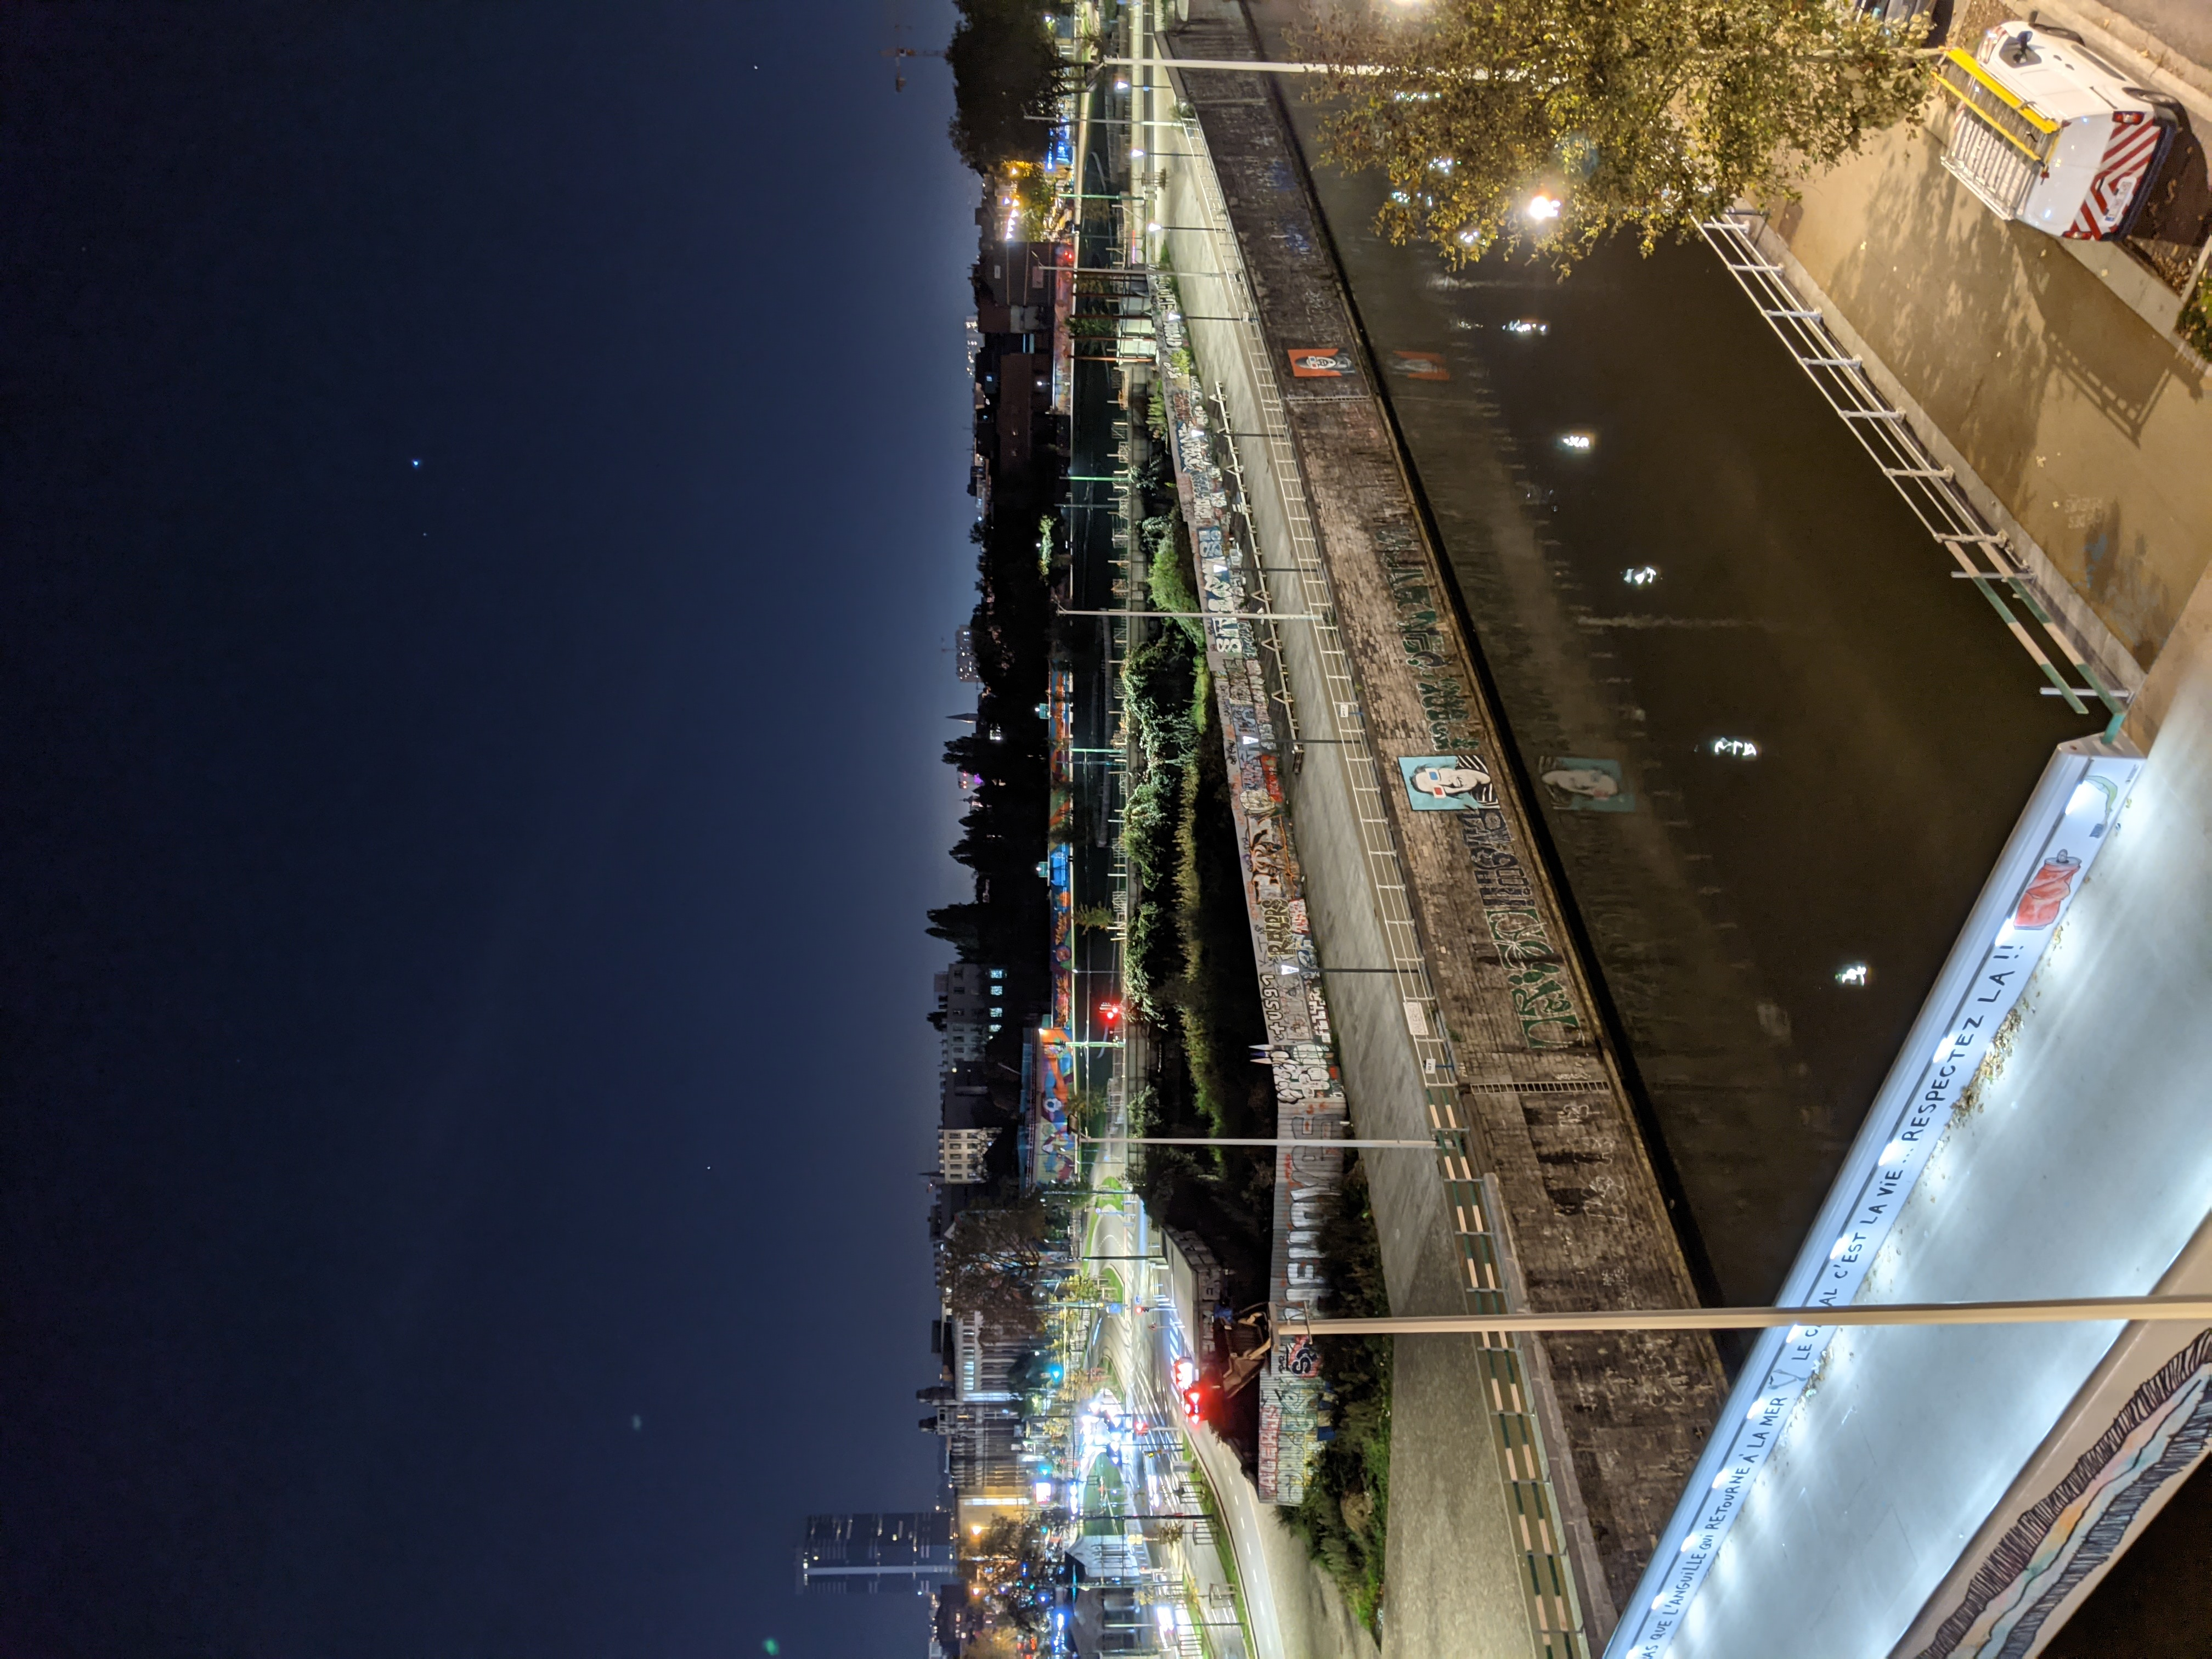
\includegraphics[width=0.85\textwidth, angle=-90]{bxl_canal_far}
	\caption{\hl{A} Night view over Ninoofsepoort, from the rooftop of the MIMA museum. From the foreground to the background, we see: the canal over the Petite Senne; an art project from Antoine Caramalli along the canal walls; an undeveloped, overgrown, fenced off plot of land; to its left, tram lines which delimit the Sint-Jans-Molenbeek commune from Brussels Capital commune; further behind, the Ninoofsepoort Park; and the very brightly lit Rue Heyvaert.}
\end{figure}

\restoregeometry

\pagebreak

\begin{comment} 

History of the ninoofsport: 
- what it used to be, why it is now empty, when and who decided to build something on top
- interesting that this triangle of land is ambiguous on land use maps and zoning maps

What can become of ninoofsepoort:
- what does the land use map permit?
- where is the ninoofsepoort located, and what would make sense in this space? comment on the street art, that reminds everyone of the location of ninoofsepoort in molenbeek
- who are the stakeholders? the city, the residents (who are diverse), private investors
- how is it inscribed in the canal redevelopment plan? definitely part of the canal, as it is located right on it; the park will be 
- talk about gentrification of the area: was the MIMA there before (where the photo is taken from), is the park just a plan for attracting private developers?
- what are the aspirations of ninoofsepoort, and how do these integrate into the canal plan? ambiguous goals

What is planned for the left over triangle of land:
- what is the surface area of it, 
- a park was already developed: but for who? minimal infrastructure and furniture, although very well used by molenbeek residents
- was the park part of the plan to attract investors to the plot of land in question?

Relation to course
- investment/disinvestment?
- part of the canal project, and the long park project, which is a gentrification of molenbeek? 

Other notes:
- Citizen Participation? Consultations citoyennes - citizen participation\marginpar{Lecture 5}

- From Urban Analysis
	- PAD: strategic plan, but also gives them the power to change the law in their own advantage; a way for the power that be to do what they want, and circumvent the laws that they usually have to respect; but also a tool for the developers to do what is efficient

- Relate to lecture 5, and gentrification: using MIMA as a regeneration project

- Keywords? Creative and capitalist destruction

- Original wording: ``véritable lieu de convivialité et d’attractivité pour toutes les populations''

\end{comment} 

The photo is a view over Ninoofsepoort, or Ninoof's Door. The name of this triangular plot of land is symbolic. Located on the edge of the Brussels' canal, it was once a city gate that provided entry to the historical city centre of Brussels. Occupied in the 20th century by warehouses and manufacturing companies, the land was left unused as the companies moved.

Today, Ninoofsepoort is at the same time a break in Brussels' urban fabric and a fantastic opportunity for development. As an area of roughly X squared kilometres, only ten minutes walking distance from the Grand Place, in a dense city with limited space, and in a neighbourhood targeted as a zone for urban renovation \parencite{perspective2020zru}, there is a lot at stake. \hl{As such, this project is high stakes for the city.}

The photo itself was taken from the rooftop of the MIMA, a museum of contemporary art opened in 2016. One of the museum's aims was to give the neighbourhood of Molenbeek a new image. An image of culture and dynamism, intended to overrule the prevailing sentiment of insecurity and fear. The faces with 3D glasses visible on the canal walls are a satirical piece by artist Antoine Caramalli, entitled `The Big Molenbeek Show'. The faces of Molenbeek are staring back in irony at those looking onto the neighbourhood, following the ``giant media circus''\parencite{antoine2016canal} after the 2016 Paris terrorist attacks carried out by Molenbeek hooligans \hl{they're terrorists not delinquent teenagers!}.

I think Caramalli, an inhabitant of Molenbeek himself, perfectly summarises the neighbourhood as the ``home of the poor, the artists, the immigrants and the tourists, fertile ground of mixity and culture''\parencite{antoine2016canal}.
This poetic description conveys Ninoofsepoort's multi-faceted \hl{politicoeconomic, sociocultural} position (political, social, economic, cultural, touristic) with many actors (\hl{includin'} inhabitants, politicians, planners, private investors).

%%%% The plot of land
Part of Ninoofsepoort has been developed into a park, visible in the back of the photo. Although minimal in its furniture, the park is well used by a diversity of inhabitants and addresses the concerns over the density of the neighbourhood and its critical lack of green space.
The undeveloped plot of land, visible as overgrown shrubs surrounded by a fence covered in graffiti, is the centre of much debate. It leads us to wonder whether the park was planned for the inhabitants, or to attract private investors in a location with unrealised potential. What is to become of this land?

% Let's focus now on this particular unbuilt section of Ninoofsepoort, and ask: who are the planners and developers? What is their vision? Who are the stakeholders? What are the stakes? What would make sense, and for whom?

%%%% Ninoofsepoort Development plans
In 2016, the government mandated perspective.brussels, an NGO, to evaluate the land and plan its development \parencite{diagnosticNinove}. Perspective formulated a goal for Ninoofsepoort - to make it ``a real place of conviviality and attractiveness for all populations'' \parencite{perspectiveNinove}. From this, three aspects stand out: conviviality, attractiveness, and all populations.

\textbf{Conviviality and Attractiveness}

Given Molenbeek's socio-economic situation, it is not hard to be critical of the PAD (Plan d'Aménagement Directeur) of Ninoofsepoort. The PAD is a tool that has the power to overrule regulations, and is being used to facilitate the plans of the private real estate developer BESIX RED. The land use has been changed to allow private housing and a height of 90 meters. The reasons for the PAD are to anchor Ninoofsepoort within Brussels' small ring, already dotted with high-rise buildings; giving Ninoofsepoort an identity; and improving
the quality of the urban space.

To these ends, three housing towers were planned. They will comprise of 270 private housing units along with 240 parking spots, and the ground floor will be open in order to create a cohesive urban fabric. None of the units will be social housing, and the mere plan for so much parking implies who will move in - a population who needs a car on a regular basis to get to work - and confirms the ambitions of BESIX RED to attract a new class. 
% Not to mention the hypocrisy, because it does not respond at all to the city's goal of promoting soft mobility.

\textbf{All populations}

The plans promote open, public space on the ground floor of the towers, with metropolitan equipment such as socio-cultural infrastructure and daycares. But for whom is this space, and this equipment? \hl{In light of the fact that the current population is lower-class} How will public and private spaces be developed, in order to facilitate diverse uses and populations? Perversely, this promotion for diversity, and the creation of the Ninoofsepoort park, encourage gentrification by attracting real estate developers like BESIX RED and middle to upper classes who are the only ones able to buy the new housing units.

\hl{Tie this back to the main argument somehow, eg. given Molenbeek's need for public investments...} So who is represented in ``all the populations''? Molenbeek is one of the poorest neighbourhoods of Brussels, one of the densest in Europe, and in desperate need of green and public spaces, and public equipment \parencite{ieb2019ninove}. \sout{The neighbourhood is a real challenge for the local government, no less because of its high levels of unemployment (25.4\% compared to the regional average of 18.65\% \parencite{monitoring2018chomage}).} Given that the towers are from a private company, and won't have any social housing, shows that the plan never aimed to include the population of Molenbeek, who could not afford the units. The argument of social mix, modernisation, and a supra-local vision prevailed.

This development is also a stark contrast to the resident's demands for their neighbourhood, when they were consulted in 2014 $\rightarrow$ maybe add this

Investing money in a disadvantaged neighbourhood tends to accelerate gentrification and displacement if there are no policies to reduce unemployment, and improve living conditions for existing residents.
Moreover, Ninoofsepoort is being used as a strategic site to integrate a multitude of projects that are part of the Canal Plan. These plans, like the PAD Heyvaert, will further displace residents and especially local businesses important to the area, like the car dealerships in Rue Heyvaert.
%including Contrats de Quartiers Durables, Masterplan Molenbeek, Plan Canal, and Contrats de Renovation Urbaine. These plans, like the PAD Heyvaert, will further displace residents and especially local businesses like the car dealerships in Rue Heyvaert. 

\textbf{Hope for the Right to the City}

this photo encapsualtes the failure of brussels city to address the failures of brussels cit
\hl{Given the above, it is clear\dots}

Let's circle back to Perspective's goal for Ninoofsepoort, to make it ``a real place of conviviality and attractiveness for all populations''. Given what we now know about the project, it is clear that there is no intention to address the aspirations and concerns of the people who currently live in the area, but rather, to cater to the aspirations of the middle and upper classes.
% The project, inscribed in the broader canal redevelopment scheme, is a state-led initiative to rebrand the area and make it attractive for a new population with better means.

The location's extremely attractive potential makes it vulnerable to investors. For the city, it is equally attractive to sell or lease the land, thus reaping the benefits of taxation and income from wealthier residents. But would they really be \textit{benefits}? Trickle down effects have long been disproven \parencite{biden2018speech}. Maybe, the neighbourhood would better benefit from direct public investments in employment and education. And perhaps worst of all, the new investments will further gentrify the neighbourhood and displace the current inhabitants who would never profit from the investments.
The vicious cycle of investment, gentrification, and displacement will perpetuate.

After a ``massive citizen mobilisation'' against speculation... $\rightarrow$  elaborate

\parencite{https://www.ieb.be/Porte-de-Ninove-bientot-une-victoire-contre-la-speculation-fonciere-et-pour-le}

%%%% Conclusion

Ninoofsepoort was an opportunity for the Brussels' government to show more ambition in the social housing developments, given the enormous demand and embarrassing supply. Unfortunately, it fell victim to ``Bruxellisation'', where the interests of private investors are prioritised over those of local inhabitants, justified by the necessity to modernise. 

Even if the housing development is not directly destroying or displacing, it contributes to the gentrification of Molenbeek. It will raise the attractiveness of the area, thus rising prices, and displacing people and businesses who either cannot afford the new rent or are forced out for the sake of urban regeneration.

\pagebreak

\printbibliography 

\end{document}
